% !TeX spellcheck = en_US
\chapter{Theory and methodology}%
As mentioned in previous sections, forming a virtual experiment platform 
is necessary for investigating the temperature estimation algorithm. So, a virtual 
experiment platform is developed based on Planks'law, then, a virtual multi-spectral 
pyrometer is applied to obtain the digital value (also called image). 


\section{Physical value of radiation}%
Radiation is emitted from any object with a temperature above $0 \, \text{K}$. In equation \ref{eq: radiation_pv}
can be found, that the radiation depends on the black body radiation $B(\lambda, T)$ 
and emissivity $\varepsilon(\lambda, T)$. Both value are temperature $T$ and wavelength $\lambda$ 
dependent.

\begin{equation}
    \label{eq: radiation_pv}
    L(\lambda, T) = B(\lambda, T) \cdot \varepsilon (\lambda, T)
\end{equation}


By Plank's Law, black body radiation can be described in equation \ref{eq: planks_law}, 
with absolute temperature $T$, wavelength $\lambda$, speed of light $c$, Plank 
constant $h$ and Boltzmann constant $k_B$. Black body radiation is irrelevant 
to the material itself, all materials at the same temperature have the same spectral 
black body radiation.

\begin{equation}
    \label{eq: planks_law}
    B(\lambda, T) = \frac{{2hc^2}}{{\lambda^5}} \cdot {\left[{\exp\left(\frac{{hc}}{{\lambda k_B T}}\right) - 1}\right]}^{-1}
\end{equation}


On the contrary, emissivity varies from material to material. It is the 
ratio of the actual spectral intensity emitted by the object to the spectral 
intensity of the black body radiation.

\begin{figure}[htbp]
    \centering
    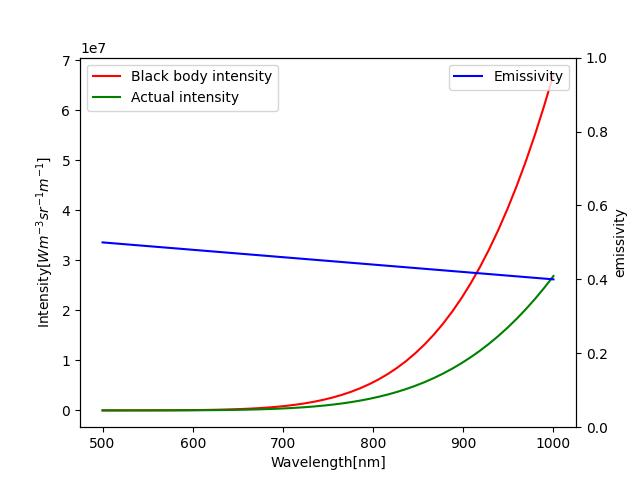
\includegraphics[width = 0.8\textwidth]{figures/real_radiation.jpg}
    \caption{Black body radiation, emissivity and real radiation of an example
    material at $1000K$}
    \label{fig: black_body_radiation}
\end{figure}


In Fig.\ref{fig: black_body_radiation} can be found, that the real spectral 
intensity of a material is lower than the black body spectral intensity. Since 
the value of emissivity of a normal material is normally in the range of 0 to 1. 

\section{Integration method}%
why we use integration model, we also used linear model for validation
%
%
\section{Digital value of radiation}%

%
%

\section{Temperature estimation algorithm}


\section{Used model in validation}%

%
%
